\documentclass{article}
\usepackage{tikz}
\usepackage{graphicx}
\usetikzlibrary{mindmap,positioning}

\begin{document}

\section{Izbira modela}
\subsection{Osrednja arhitektura}
\begin{itemize}
    \item{Pristopi so bili ovrednoteni posamično, s predpostavko medsebojne neodvisnosti (zaradi zahtevnosti treniranja)}
    \item{Modeli vrednoteni relativno med vozlišči na istem nivoju grafa}

    \item{Označbe metod:}
    \begin{itemize}
        \item{Siva - nepreizkušeno}
        \item{Zelena - izbrano za končni model}
        \item{Rdeča - neizbrano/slabše}
        \item{Modra - primerjava ni nujno primerna}
        \item{Rumena - ne predstavlja opazne izboljšave}
    \end{itemize}
\end{itemize}

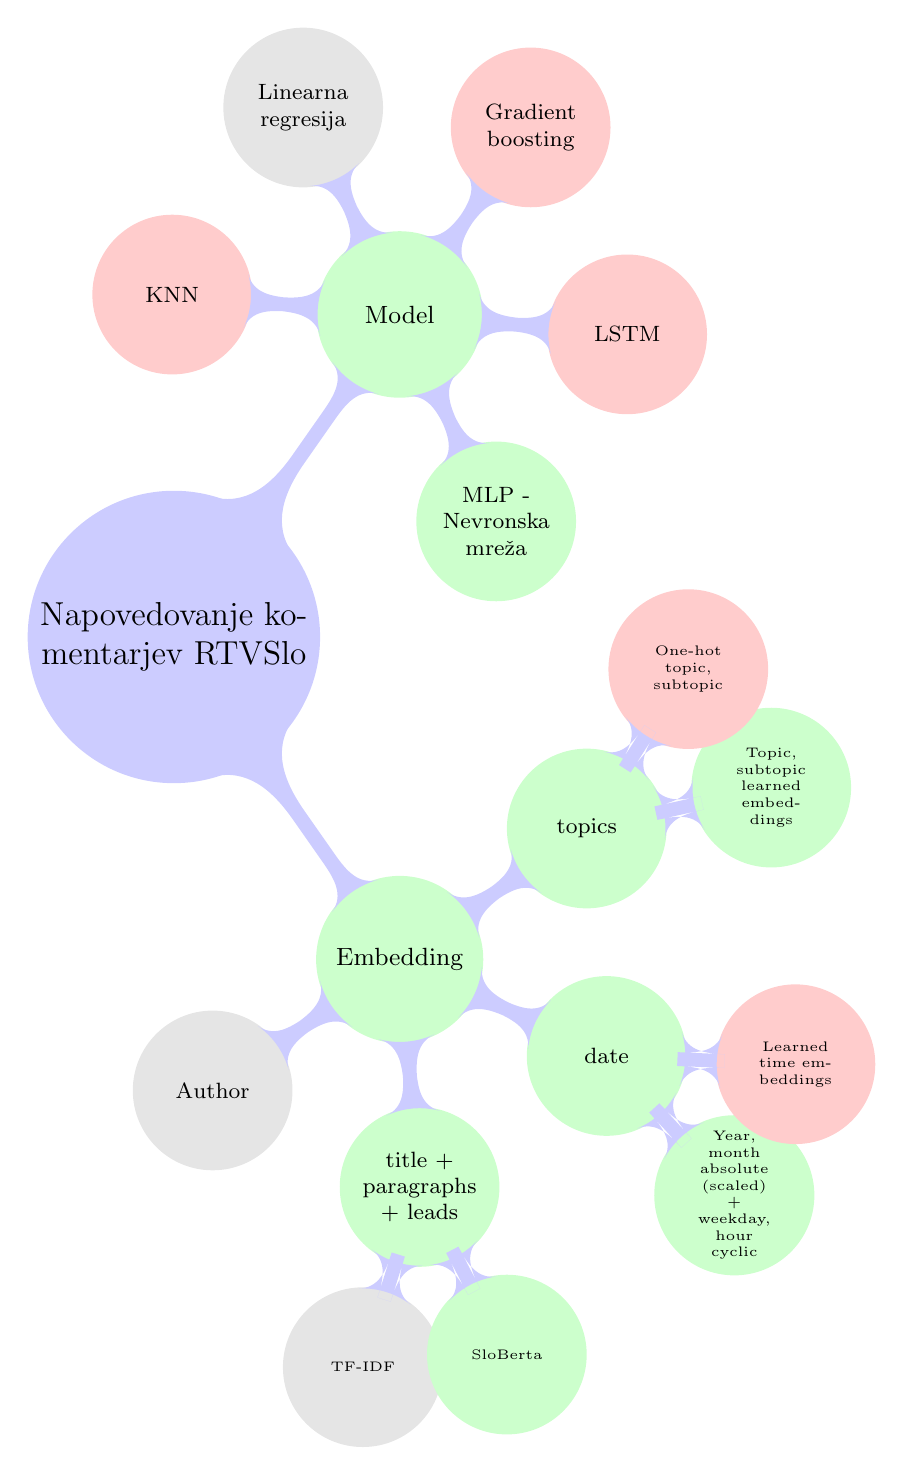
\begin{tikzpicture}[mindmap,
    every node/.style={concept, draw, circle, thick, text=black, minimum size=2cm},
    concept color=blue!20,
    grow cyclic,
    level 1/.append style={sibling angle=110},
    level 2/.append style={sibling angle=60},
    level 3/.append style={sibling angle=45},
    ]
  \node {Napovedovanje komentarjev RTVSlo}
      child { node[concept color=green!20] {Embedding}
          child { node[concept color=gray!20] {Author} }
          child { node[concept color=green!20] {title + paragraphs + leads}
              child { node[concept color=gray!20] {TF-IDF} }
              child { node[concept color=green!20] {SloBerta} }
          }
          child { node[concept color=green!20] {date}
              child { node[concept color=green!20] (datetime) {Year, month absolute (scaled) + weekday, hour cyclic} }
              child { node[concept color=red!20] {Learned time embeddings} }
          }
          child { node[concept color=green!20] {topics}
              child { node[concept color=green!20] {Topic, subtopic learned embeddings} }
              child { node[concept color=red!20] {One-hot topic, subtopic} }
          }
        }
      child { node[concept color=green!20] {Model}
          child { node[concept color=green!20] {MLP - Nevronska mreža} }
          child { node[concept color=red!20] (lstm) {LSTM} }
          child { node[concept color=red!20] {Gradient boosting} }
          child { node[concept color=gray!20] (linreg) {Linearna regresija} }
          child { node[concept color=red!20] (knn) {KNN} }
        };

\iffalse
\node[draw=none, fill=none, text=black, above left=-15mm and 5mm of knn] {
  \scriptsize
  \begin{itemize}
    \setlength\itemsep{1pt}        % spacing between items
    \setlength\parskip{0pt}        % paragraph spacing
    \setlength\parsep{0pt}         % spacing between item and paragraph
    \item ugotovitev: \\ \textbf{Napoved primitivnega modela je $\approx 36\mathrm{MAE}$}
  \end{itemize}
};
\fi

\end{tikzpicture}

\section{Vrednotenje}
\begin{itemize}
    \item Med treniranjem je model vrednoten na validacijski podmnožici učne množice (95\% training / 5\% validation) in uporablja early stopping glede na MAE na validacijski množici. Končni model je evalviran na testni množici na tekmovalnem strežniku.
    \item Lokalno so bili modeli evalvirani tudi na testni podmnožici iz učne množice, ki ni bila vključena v trening.
    \item Maksimiziramo MAE, vendar so bili modeli primerjani tudi po distribuciji napovedi ..., ki pa se po navadi neposredno pozna na MAE.
\end{itemize}
Za končni model je bil izbran ensemble treh enakih MLP modelov, ki delujejo nad bert vložitvami s topici, subtopici ter časovnimi vložitvami. 
\subsection{Izbira hiperparametrov}
Hiperparametri modela:
\begin{itemize}
    \item loss function - L1 loss / HuberLoss
    \item batch size - 150
    \item learning rate - 1e-4
    \item weight decay - 1e-3
    \item dropout - 0.1
    \item hidden layer dimension - 1024
\end{itemize}
Hiperparametri so bili izbrani s pomočjo grid searcha. Napovedi z izbranim modelom se kljub istemu seedu, s ponovnimi zagoni razlikujejo, zato je potrebno hiperparametre evalvirati na poveprečju večih zagonov. Uporabljeno je bilo 3kratno prečno preverjanje.
\section{Razlaga modela}

%\includegraphics[scale=0.7]{imgs/model.png}
\subsection{SHAP}
\begin{center}
%\includegraphics[scale=0.7]{imgs/shap_values.png}
\newpage
%\includegraphics[scale=0.7]{imgs/shap_importance.png} \\
%\includegraphics[scale=0.7]{imgs/shap_table.png} \\
%\includegraphics[scale=0.5]{imgs/topic_shap.png} \\
%\includegraphics[scale=0.5]{imgs/subtopic_shap.png} \\
\end{center}

\section{Dodatne slike in diagrami}

\end{document}
